\documentclass[10pt,conference]{IEEEtran}
\usepackage{cite}
\usepackage{amsmath,amssymb,amsfonts}
\usepackage{algorithmic}
\usepackage{graphicx}
\usepackage{textcomp}

\title{ABC: Action-Based Test Carving}

\author{\IEEEauthorblockN{Alessio Gambi}
\IEEEauthorblockA{\textit{University of Passau} \\
%\textit{name of organization (of Aff.)}\\
Passau, Germany \\
alessio.gambi@uni-passau.de}%
}


\begin{document}

\maketitle

\begin{abstract}
\end{abstract}

\section{Evaluation}

\textbf{Goal of the evaluation} Show the usefulness of test carving

\subsection{Test Subjects}

% Is this really required? Can't we simply say they always match ?
\subsection{Results}
\begin{table*}
\caption{Code coverage - Does this make sense?}
\end{table*}

\begin{figure*}[t]
\centering
\begin{minipage}[b]{.45\textwidth}
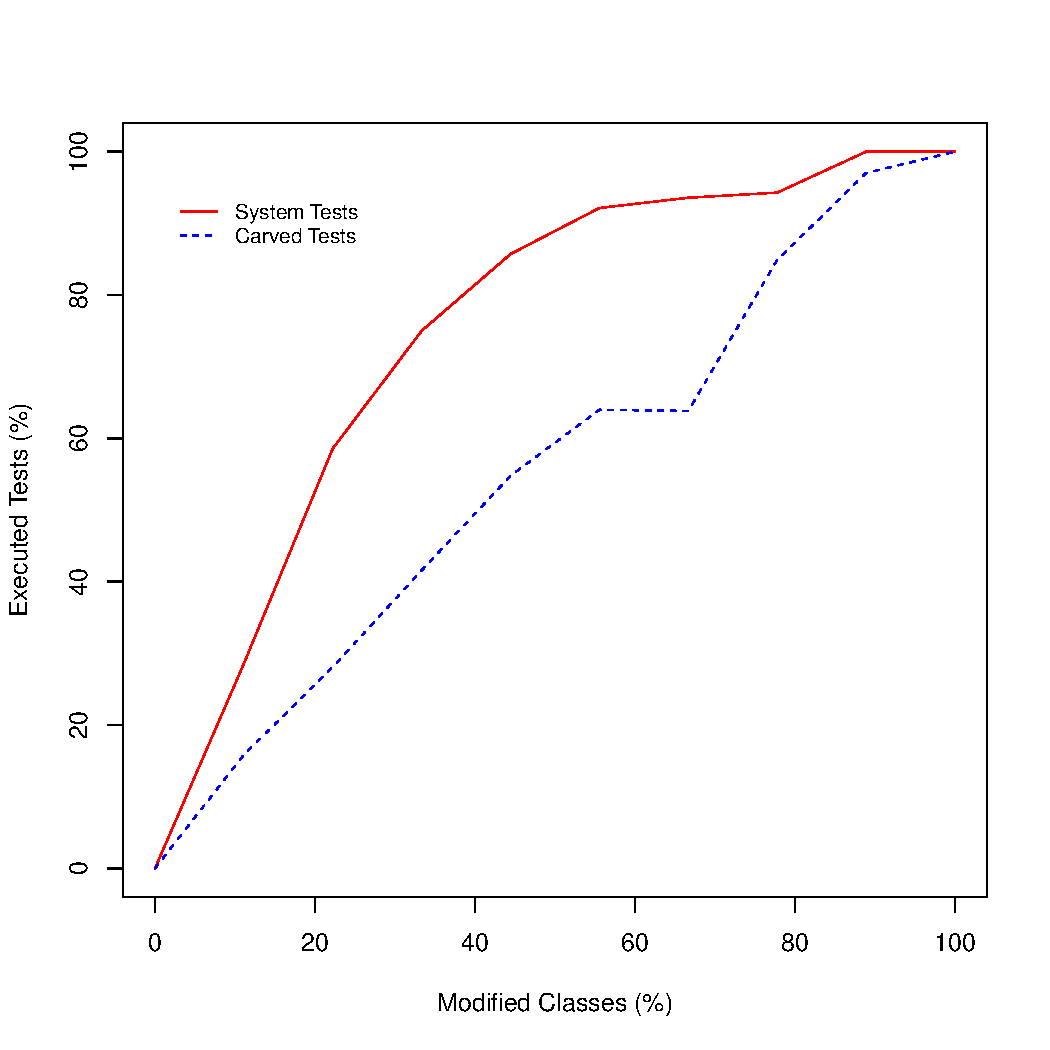
\includegraphics[width=\columnwidth]{figures/employee}
\caption{Test Regression Selection - Employee}
\end{minipage}\hfill
\begin{minipage}[b]{.45\textwidth}
\includegraphics[width=\columnwidth]{figures/hotelme}
\caption{Test Regression Selection - Hotel Reservation System}
\end{minipage}
\end{figure*}



\subsection{Discussion}


\end{document}